\section{Building Quantum Circuits}

Building Quantum circuit using Qiskit is very easy. Qiskit is written in the Python Programming Language and thus it can be installed
by the user from its official Python Package Index using \verb|pip| \cite{QiskitPIP}. After installing the dependencies we can
\verb|import| the Quantum Circuit class from the Qiskit API. Then we can instanciate an \verb|QuantumCircuit| object with a number
of qubits and bits. We can then apply various Quantum gates onto the circuit. For example we can build a Quantum circuit with two
qubits, $q_0\text{ and }q_1$, and then apply a Hadamard gate on $q_0$ and an $X$ gate on $q_1$.

\begin{listing}[ht]
    \centering
    \begin{minted}{python3}
        from qiskit import QuantumCircuit
        
        circuit = QuantumCircuit(2)
        
        circuit.h(0)
        circuit.x(1)
        
        print(circuit.draw("latex_source"))
    \end{minted}
    \centering
    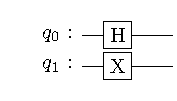
\includegraphics{images/4_Qiskit/example_circuit_1.pdf}
    \caption{Building a simple Quantum circuit and its diagram compiled from its \LaTeX source code}
\end{listing}


Qiskit also provides us with functions that can visualize a circuit. Every QuantumCircuit object has a member function for
printing the circuit using many different output methods like: ASCII text (great if you are in a CLI enviroment), as a Matplotlib
plot if you are in an interactive Python enviroment or output the \LaTeX source code of the circuit diagram for the highest resolution.